

编码 $ \left\{\begin{array}{l}\text { 信源编码 }\left\{\begin{array}{l}\text { 减少冗余度,即把信源输出符号序列变换为最短的 } \\ \text { 把相关性降低,使各符号尽量独立 } \\ \text { 码字不能改变信源所携带的最低的信息 }\end{array}\right.\\ \text{信道编码}\end{array}\right. $

\begin{figure}[h]
    \centering
    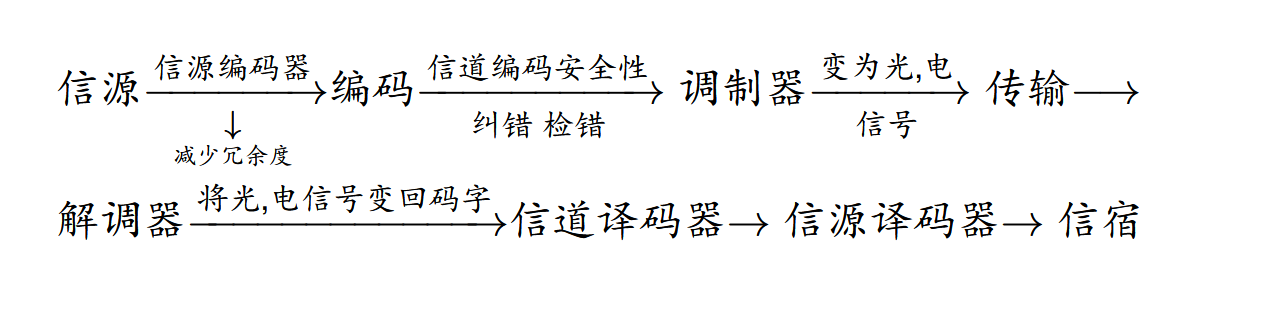
\includegraphics[width=1\linewidth]{image/2.png}
    %\caption{Enter Caption}
\end{figure}

\section{信源编码问题}
\subsection{信源编码}
\begin{definition}
     信源序列: 设 $ \mathscr{S}=\{\mathscr{X}, p(x)\} $ 为信源, 其中 $ \mathscr{X} $ 为信息字母表, $ p(x), x \in \mathscr{X} $ 为消息字母表上的概率分布,将 $ \mathscr{X} $中的信源字母进行分组, 记为 $ x_{1}^{(n)}, x_{2}^{(n)}, \cdots, x_{L}^{(n)} $.其中 $ x_{i}^{(n)}=\left\{x_{i 1}, x_{i 2}, \cdots, x_{i n}\right\}, i=1, \cdots, L, x_{i j} \in X $, $ j=1, \cdots, n $. 每个 $ x_{i}^{(n)} $ 的概率分布记为 $ p_{i}^{(n)} $,记 $ \mathscr{S}^{n}=\left\{\mathscr{X}^{n}, p^{(n)}\left(x^{(n)}\right)\right\} $ 称其为信源序列.
\end{definition}

\begin{remark}

(1)发送消息时通常不是一个一个信源字母进行发送, 而是把它们分组变为信源序列后进行发送, 可以减少发送次数.

(2)例: $ \mathscr{X}=\{0,1\}, p(0)=p, p(1)=1-p $,
$x_{1}^{(3)}=001, x_{2}^{(3)}=111, x_{3}^{(3)}=101 $,
 则  $p_{1}^{(3)}=(p, p, 1-p), p_{2}^{(3)}=(1-p, 1-p, 1-p) ,
p_{3}^{(3)}=(1-p, p, 1-p)$.
于是信源序列为 $ \left\{\mathscr{X}^{3}, p^{(3)}\left(x^{(3)}\right)\right\} $.
\end{remark}


\begin{definition}
    记 $ \mathscr{U} $ 和 $ \mathscr{U}^{m} $ 分别为信道的输入信号字母表和输入信号字母表序列, $ \mathscr{U}^{*}=\bigcup\limits_{m=1}^{\infty} \mathscr{U}^{m} $ 为由全体信号字母串所组成的集合,其中 $ \mathscr{U}^{m} $是全体在 $ \mathscr{U} $ 上取值的 $ m $ 维向量的集合,则称映射 $ f: \mathscr{X}\left(\mathscr{X}^{n}\right) \rightarrow \mathscr{U}^{*} $ 为信源编码 $ f $.
\end{definition}
\begin{remark}

    (1) $ f: \mathscr{X}^{n} \rightarrow \mathscr{U}^{*} $ 即 $ f $ 可把 $ n $ 长的消息序列变为信号序列(可以不等长);
    
(2)信源编码的基本要求是编码运算的可还原性,即可唯一的把码字还原为消息.

(3)编码可还原性的一个必要条件是编码运算 $ f $ 的 $ 1-1 $ 性(显然,后面举例说明 $ 1-1 $ 性是必要条件而不是充要条件)

\end{remark}

\begin{definition}
$ 1-1 $ 码: 如果对于 $ \forall x \neq x^{\prime} \in \mathscr{X} $, 都有 $ f(x) \neq f\left(x^{\prime}\right) $, 则称 $ f $ 是一个1 - 1 编码,也称 $ f $ 满足 $ 1-1 $ 性.
\end{definition}
\begin{remark}
 $ 1-1 $ 码不一定是可还原码,后面举例说明.
\end{remark}

\subsection{定长编码与变长编码}
1.定长编码与变长编码
\begin{definition}
    若编码 $ f: \mathscr{X}^{n} \rightarrow \mathscr{U}^{m} $, 其中 $ m, n $ 是两个固定的正整数, 则称 $ f $ 是一个定长编码, 即把 $ \left(x_{1}, \cdots, x_{n}\right) \rightarrow\left(u_{1}, \cdots, u_{m}\right) $ (码字长度固定)若 $ f: \mathscr{X} \rightarrow \mathscr{U}^{*} $, 称 $ f $ 为变长编码(码字长度不固定)
\end{definition}
2. 扩张编码与唯一可译码
\begin{definition}
    (1)设 $ f: \mathscr{X}\left(\mathscr{X}^{n}\right) \rightarrow \mathscr{U}^{m} $ 定长编码. 记 $ x^{(k n)}=\left(x_{1}^{(n)}, x_{2}^{(n)}, \cdots, x_{k}^{(n)}\right) $, 其中 $ x_{j}^{(n)}=\left(x_{j 1}, \cdots, x_{j n}\right) $ $ j=1,2, \cdots, k $. 对任何的 $ k=1,2,3, \cdots $, 定义
$$
f^{*}\left(x^{(k n)}\right)=\left(f\left(x_{1}^{(n)}\right), f\left(x_{2}^{(n)}\right), \cdots, f\left(x_{k}^{(n)}\right)\right)
$$
则称 $ f^{*} $ 是 $ f $ 的扩张编码. 这时 $ f^{*} $ 是一个从 $ \left(\mathscr{X}^{n}\right)^{*} $ 到 $ \mathscr{U}^{*} $ 的映射.

(2) 设 $ f $ 是 $ \mathscr{X} $ 到 $ \mathscr{U}^{*} $ 的变长码, $ x^{(k)}=\left(x_{1}, x_{2}, \cdots, x_{k}\right) $ 是一个消息字母串, 对任何 $ k=1,2,3, \cdots $, 定义
$$
f^{*}\left(x^{(k)}\right)=\left(f\left(x_{1}\right), f\left(x_{2}\right), \cdots, f\left(x_{k}\right)\right)
$$
称 $ f^{*} $ 是 $ f $ 的扩张编码. 这时 $ f^{*} $ 是一个从 $ \mathscr{X}^{*} $ 到 $ \mathscr{U}^{*} $ 的映射.

(3) 无论是定长编码还是变长编码, 它们的扩张 $ f^{*} $ 都是从 $ \left(\mathscr{X}^{n}\right)^{*} $ (或 $ \mathscr{X}^{*} $ ) 到 $ \mathscr{U}^{*} $ 的映射.如果 $ f^{*} $ 是一个 $ 1-1 $ 映射,那么我们称 $ f $ 是一个唯一可译码(或可还原码).
\end{definition}

3. 唯一可译码与 $ 1-1 $ 码的关系
\begin{theorem}
 (1)无论是定长编码还是变长编码, 唯一可译码必是 $ 1-1 $ 码.\\
(2)如果 $ f $ 是一个 $ 1-1 $ 定长码,那么 $ f $ 是一个唯一可译码.\\
(3)唯一可译的变长码 $ f $ 一定是 $ 1-1 $ 码,反之不然.
\end{theorem}
\begin{proof}
    (1) 用反证法.若 $ f $ 不是 $ 1-1 $ 码, 由扩张编码的定义 $ f^{*} $ 也不是一一映射,与 $ f $ 是唯一可译码矛盾,故 $ f $ 必是 $ 1-1 $ 码.

(2) 证明 $ f $ 是唯一可译码, 只需证明 $ f^{*} $ 是一一映射( $ f $ 是定长码 ) ,即 $ f^{*} $ 是单射.设 $ x^{(k n)} \neq y^{(k n)} $, 那么必有一个 $ j \in\{1,2, \cdots, k\} $ 使 $ x_{j}^{(n)} \neq y_{j}^{(n)} $, 因为 $ f $ 是 $ 1-1 $ 码, 所以必有 $ f\left(x_{j}^{(n)}\right) \neq f\left(y_{j}^{(n)}\right) $, 从而
$$
\left(f\left(x_{1}^{(n)}\right), f\left(x_{2}^{(n)}\right), \cdots, f\left(x_{k}^{(n)}\right)\right) \neq\left(f\left(y_{1}^{(n)}\right), f\left(y_{2}^{(n)}\right), \cdots, f\left(y_{k}^{(n)}\right)\right),
$$
即 $ f^{*}\left(x^{(k n)}\right) \neq f^{*}\left(y^{(k n)}\right), f^{*} $ 是 $ 1-1 $ 映射(单射). 从而 $ f $ 是唯一可译码.

(3) 由(1)知唯一可译的变长码 $ f $ 一定是 $ 1-1 $ 码. 下面举例说明对于变长码来说, $ f $ 是 $ 1-1 $ 码, $ f $ 不一定是唯一可译码,即 $ f^{*} $ 不一定是 $ 1-1 $ 映射.

取 $ \mathscr{X}=\{a, b, c\}, \mathscr{U}=\{0,1\} $, 令 $ f(a)=0, f(b)=01, f(c)=001 $.则 $ f $ 是一个 $ 1-1 $ 变长码,但 $ f $ 不是唯一可译码.

事实上, $ f^{*}(c)=(0,0,1), f^{*}(a, b)=(f(a), f(b))=(0,0,1) $, $ (a, b) \neq c $, 但 $ f^{*}(a, b)=f^{*}(c) $, 因此 $ f^{*} $ 不是 $ \mathscr{X}^{*} $ 到 $ \mathscr{U}^{*} $ 的 $ 1-1 $ 映射,故 $ f $ 不是唯一可译码.
\end{proof}

4. 一些概念

(1)二元码:如果信号字母集 $ \mathscr{U}=\{0,1\} $, 则称相应的码(定长或者变长) 为二元码,称 $ \mathscr{U}_f=\{f(x) \mid x \in \mathscr{X}\} $ 为码元集,记作 $ C=\mathscr{U}_{f}=\left\{c_{1}, c_{2}, \cdots, c_{a}\right\} $,其中 $ c_{i}=f\left(x_{i}\right) $.

(2) 记 $ \ell_{f}(x) $ 为码字 $ f(x) $ 的长度, $ \ell_{i}=\ell_{f}\left(x_{i}\right) $ 为 $ x_{i} $ 对应的码字 $ f\left(x_{i}\right) $ 的长度,此时码元集 $ C=\mathscr{U}_{f}=\left\{u_{i}^{\left(\ell_{i}\right)}, i=1,2, \cdots, a\right\} $,
$$
u_{i}^{\left(\ell_{i}\right)}=\left(u_{i 1}, u_{i 2}, \cdots, u_{i \ell_{i}}\right)=f\left(x_{i}\right), u_{i j} \in \mathscr{U}
$$
此时有 $ C=\left\{c_{1}, c_{2}, \cdots, c_{a}\right\}=\left\{u_{1}^{\left(\ell_{1}\right)}, u_{2}^{\left(\ell_{2}\right)} \cdots, u_{a}^{\left(\ell_{a}\right)}\right\} $,如上例 $ C=\mathscr{U}_{f}=\{0,01,001\}, \ell_{1}=1, \ell_{2}=2, \ell_{3}=3 $,因此有
$$
C=\left\{u_{1}^{(1)}, u_{2}^{(2)}, u_{3}^{(3)}\right\} \text {. }
$$
\subsection{信源变长码的编码问题}

\begin{definition}[变长编码 $ f $ 的平均码长]
    设 $ \mathscr{S}=\{\mathscr{X}, p(x)\} $ 是一个信源, $ f $ 是一个变长编码, 对于 $ \forall x \in \mathscr{X}, f(x) \in \mathscr{U}^{*} $, 记 $ \ell_{f}(x) $ 是 $ f(x) $ 的向量长度, 定义 $$ L(\mathscr{S}, f)=\sum_{x \in \mathscr{X}} p(x) \ell_{f}(x) $$ 为变长编码 $ f $ 的平均码长.
\end{definition}
\begin{remark}
    (1)平均码长小占存储空间少,易于传输.
(2) 平均码长与概率分布密切相关.
\end{remark}

\begin{example}
    考虑信源 $ \mathscr{S}=\left(\begin{array}{cccc}a & b & c & d \\ \frac{2}{17} & \frac{2}{17} & \frac{9}{17} & \frac{4}{17}\end{array}\right) \quad \mathscr{X}=\{a, b, c, d \}$.
    
    $ \mathscr{U}=\{0,1\} $ 是二进制信号字母表, $ f_{1}, f_{2} $ 是两个编码方案, 
    $$ f_{1}: \quad f_{1}(a)=11, \quad f_{1}(b)=0, \quad f_{1}(c)=100, f_{1}(d)=10 $$
    $$ f_{2}: \quad f_{2}(a)=01010, \quad f_{2}(b)=00, \quad f_{2}(c)=10, \quad f_{2}(d)=11 $$

计算它们的平均码长
$$
\begin{aligned}
&L\left(\mathscr{S}, f_{1}\right)=\frac{2}{17} \times 2+\frac{2}{17} \times 1+\frac{9}{17} \times 3+\frac{4}{17} \times 2=\frac{41}{17} \\
&L\left(\mathscr{S}, f_{2}\right)=\frac{2}{17} \times 5+\frac{2}{17} \times 2+\frac{9}{17} \times 2+\frac{4}{17} \times 2=\frac{40}{17}
\end{aligned}
$$
\end{example}

\begin{definition}[变长信源编码问题]
    如果 $ \mathscr{S}=\{\mathscr{X}, p(x)\} $ 是一个给定的信源, 变长信源编码问题是: 求一个唯一可译的变长码 $ f $, 使 $ L(\mathscr{S}, f) $ 最小, 即求唯一可译的变长码 $ f_{0} $, 使得 $ f_{0} $ 相对于其他唯一可译变长码 $ f $,总有
$$
L\left(\mathscr{S}, f_{0}\right) \leq L(\mathscr{S}, f)
$$

这时, 称 $ f_{0} $ 为 $ \mathscr{S} $ 的最优变长码.
\end{definition}
\subsection{信源序列的定长编码问题}

记 $ \mathscr{S}^{n}=\left\{\mathscr{X}^{n}, p^{(n)}\left(x^{(n)}\right)\right\}, n=1,2,3, \cdots $, 是信源序列. $ \mathscr{U} $ 是输入信号字母表, $ \mathscr{U}^{(m)} $ 是 $ \mathscr{U} $ 的 $ m $ 维乘积空间,即 $ \mathscr{U}^{(m)}=\left\{\left(u_{1}, \cdots, u_{m}\right) \mid u_{i} \in \mathscr{U}\right\} $. 定长编码 $ (f, g) $ 分别是 $ f: \mathscr{X}^{n} \rightarrow \mathscr{U}^{m}, \quad g: \mathscr{U}^{m} \rightarrow \mathscr{X}^{n} $

记 $ \xi^{(n)} $ 是由 $ \mathscr{S}^{n} $ 决定的随机变量.


\begin{definition}[编码的平均误差和可达速率]
    (1) 对于固定的信源 $ \mathscr{S}^{n} $, 与编、译码函数 $ (f, g) $, 它们的平均误差为
$$
e_{n}(f, g)=P_{r}\left\{\xi^{(n)} \neq g\left(f\left(\xi^{(n)}\right)\right)\right\}
$$

(2)记 $ C=\mathscr{U}_{f}^{(m)}=\left\{f\left(x^{n}\right) \mid x^{(n)} \in \mathscr{X}^{n}\right\} $ 为定长编码码字的集合,称 $ V_{n}=\left|\mathscr{U}_{f}^{(m)}\right| $ 为编码的信号体积,而称
$$
R_{n}=\frac{1}{n} \log \left(v_{n}\right)=\frac{1}{n} \log \left|\mathscr{U}_{f}^{(m)}\right|
$$
为编码 $ f $ 的码率.
\end{definition}
\begin{remark}

    (1) 记 $ \mathscr{U}=\left\{u_{1}, u_{2}, \cdots, u_{k}\right\} $, 码字长度为 $ m $. 对于 $ u_{i} \in \mathscr{U}, u_{i} $ 能携带的最大信息量为 $ \log _{2} k $.
    
(2)则 $ m $ 长码字所提供的最大信息量为 $ m \log _{2} k $.
\end{remark}



\begin{definition}[信源序列编码的可达速率]
    称 $ R $ 是信源序列 $ \mathscr{S}^{n} $ 的一个可达速率, $ n=1,2, \cdots $, 如果存在一个数列 $ \varepsilon_{n} \rightarrow 0 $, 当 $ n \rightarrow \infty $ 时,存在一组编码序列 $ \left(f^{(n)}, g^{(n)}\right) $ 使得以下条件成立.

(1)对任何 $ n=1,2,3, \cdots, e\left(f^{(n)}, g^{(n)}\right) \leq \varepsilon_{n} \rightarrow 0 $

(2)对任何 $ n=1,2,3, \cdots, R_{n} \leq R\left(1+\varepsilon_{n}\right) \rightarrow R $. 其中 $ R_{n}=\frac{1}{n} \log M_{n}, M_{n}=\left|\mathscr{U}_{f}^{(m)}\right| $.
\end{definition}


可达速率是指对每组编码序列 $ \left(f^{(n)}, g^{(n)}\right) $, 在误差范围内传输的平均信息量, 故定长编码问题是考虑最小可达速率, 即在误差范围内传输的的平均信息量最小值.

\begin{definition}[信源序列的最小可达速率和它的编码问题]
    对已给的信源序列 $ \mathscr{S}^{n} $, 全体可达速率的最小值,称为该信源序列的最小可达速率,信源序列的编码问题就是求它的最小可达速率.(注:每取一组 $ \left(f^{(n)}, g^{(n)}\right) $ 就有一个可达速率,去找所有的最小值)
\end{definition}

\begin{example}
     $ \mathscr{S} $ 是信源, $ \mathscr{X}=\left\{x_{1}, x_{2}, \cdots x_{5}\right\} $ 为信源字母表,对应的概率分布为 $ p_{1}=1-\varepsilon, p_{2}=p_{3}=p_{4}=p_{5}=\frac{\varepsilon}{4} \cdot \mathscr{U}=\{0,1\} $, 利用定长编码, 则码字长度至少为 3 . (否则最多有 4 个码字, 不能建立映射).码字长度为 $ n $ 的二进制编码可以有 $ 2^{n} $ 个不同的码字,$ 4=2^2<5<2^{3}=8 $.

如果采用变长编码,令
$$
f\left(x_{1}\right)=0,\left(f\left(x_{2}\right), f\left(x_{3}\right), f\left(x_{4}\right), f\left(x_{5}\right)\right)=(100,101,110,111)
$$
它的平均码长为
$$
L(\mathscr{S}, f)=(1-\varepsilon)+4 \times \frac{\varepsilon}{4} \times 3=(1-\varepsilon)+3 \varepsilon=1+2 \varepsilon,
$$
只要 $ \varepsilon<1 $, 就会有 $ L(\mathscr{S}, f)=1+2 \varepsilon<3 $. 如果 $ \varepsilon<\frac{1}{2} $, 则有 $ L(\mathscr{S}, f)=1+2 \varepsilon<2 $. 因此利用变长码可以大大压缩信源的编码长度.

$ f $ 是唯一可译码只需验证 $ f^{*} $ 是 $ 1-1 $ 映射(显然).
\end{example}


